\documentclass[fleqn]{article}
\usepackage{graphicx}
% \usepackage{polski}
\usepackage[utf8]{inputenc}
\usepackage{listings}
\usepackage{amsmath}
\usepackage{courier}
\usepackage[top=0.3in, bottom=0.8in, left=0.8in, right=0.8in, a5paper]{geometry}
\newcommand\numberthis{\addtocounter{equation}{1}\tag{\theequation}}
\renewcommand{\familydefault}{\sfdefault}

\usepackage{listings}
\usepackage{color}
 
\definecolor{codegreen}{rgb}{0,0.6,0}
\definecolor{codegray}{rgb}{0.5,0.5,0.5}
\definecolor{codepurple}{rgb}{0.58,0,0.82}
\definecolor{backcolour}{rgb}{0.95,0.95,0.92}
 
\lstdefinestyle{mystyle}{
    commentstyle=\color{codegreen},
    keywordstyle=\color{magenta},
    numberstyle=\tiny\color{codegreen},
    stringstyle=\color{codepurple},
    basicstyle=\footnotesize,
    breakatwhitespace=false,         
    breaklines=true,                 
    captionpos=b,                    
    keepspaces=true,                 
    numbers=left,                    
    numbersep=5pt,                  
    showspaces=false,                
    showstringspaces=false,
    postbreak=\raisebox{0ex}[0ex][0ex]{\ensuremath{\color{red}\hookrightarrow\space}},
    showtabs=false,                  
    tabsize=2
}
\lstset{style=mystyle}

\usepackage{color}
\definecolor{light-gray}{gray}{0.20}
\color{white}
\pagecolor{light-gray}

\begin{document}

\title{N-bodies simulation}
\author{Szymon Bugaj}

\maketitle

\begin{abstract}
A system of N material points under the force of gravity. Symulation and visualisation.
\end{abstract}

\tableofcontents



\section{Theoretical introduction}
The project is devoted to symulation and visualisation of the problem of N-bodies. 

Newtonian gravitational force between two material points is given as:
\begin{align*}
    &\vec{F_{G}} = G\frac{m_{1} m_{2}}{\|r\|^{2}}\frac{\vec{r}}{\|r\|} \\
\end{align*}

In the classical physics, the equation linking acceleration, mass and force is given as follow:
\begin{align*}
    &\vec{F} = \vec{a}m \\
\end{align*}

The relationship between the position, velocity and acceleration is given by equations:
\begin{align*}
    &v(t) = \frac{dp(t)}{dt} \\
    &a(t) = \frac{dv(t)}{dt} \\
\end{align*}

Given the position of all N particles and the speed for a given torque, using the above equations, we can calculate the location for any point at any other time.

\section{Resolution of gravity into components parallel to axis}
In the case of 2D should be considered rectangle with sides parallel to the axes X and Y, where the opposite tops are considered two of the body.

\begin{frame}
\frametitle{Resolution of gravity into components}
\begin{center}
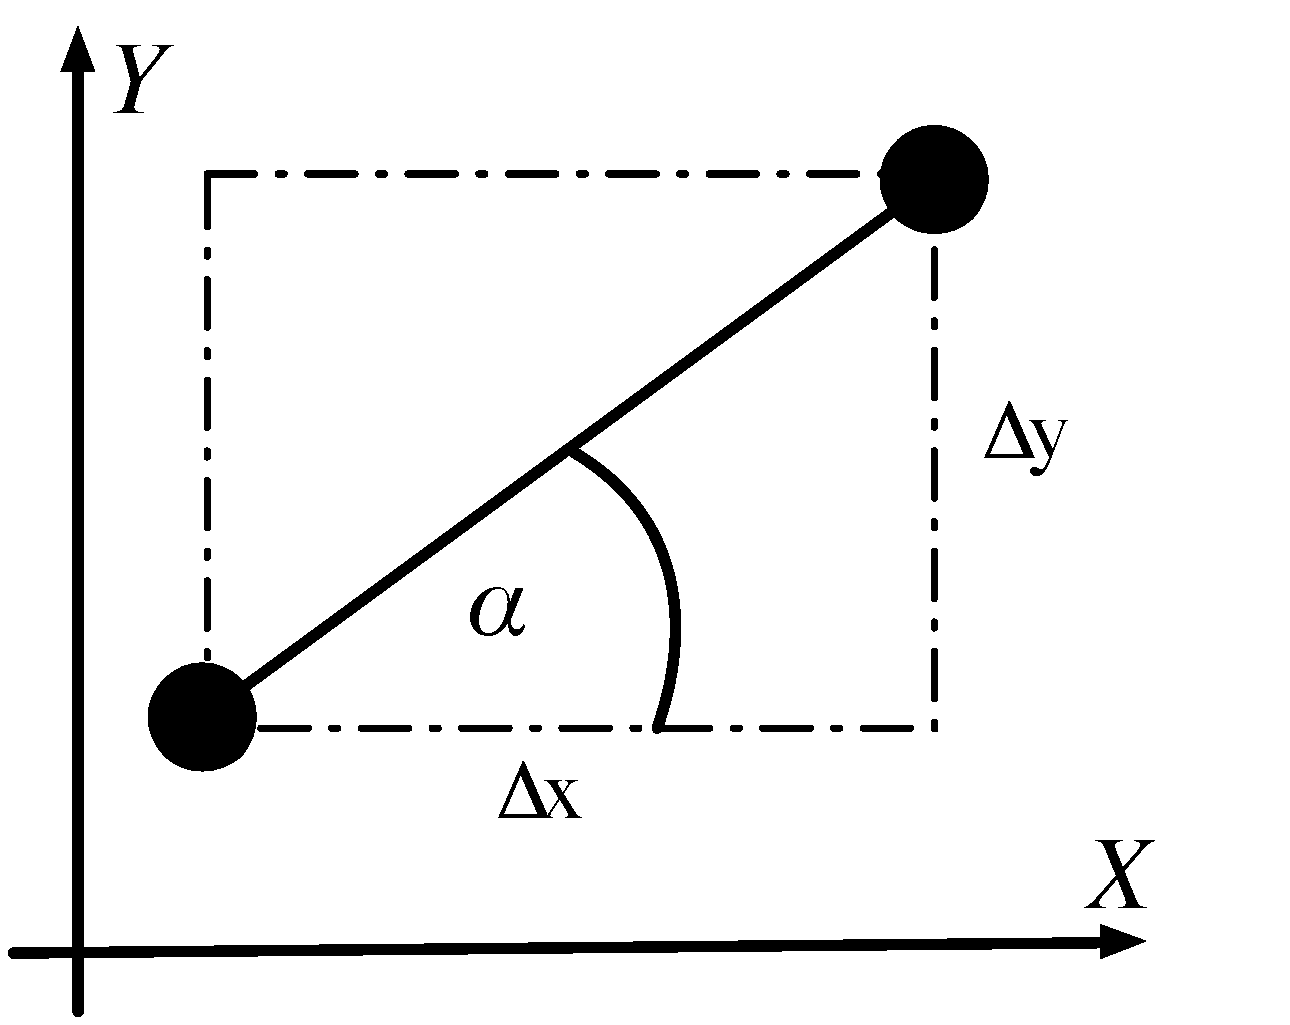
\includegraphics[width=8cm]{resolutionofgravity.pdf}
\end{center}
\end{frame}

\begin{align*}
    &a_{x}(t) = sin\alpha * a \\
    &a_{y}(t) = cos\alpha * a \\
\end{align*}

For the 3D case should be considered in an analogous manner Box (body should be at the vertices of the opposite walls at opposite corners).

\section{Numerical model}
We are interesed in position of each of a body in proceding discrete time moments. We assume, that during a smallest time unit speed, acceleration of a body is constant. All variables are updated in order: 
\begin{itemize}
    \item 1) speed
    \item 2) position
    \item 3) acceleration
\end{itemize}

What must be stressed, in consequence in calculation of update of speed is taken previous value of acceleration.

% \begin{minipage}{\linewidth}
\begin {lstlisting}[language=C++]
void NBodiesSystem::step( time_type delta_t ) {
    p_prev = p_curr;
    v_prev = v_curr;

    /*
        UPDATE v SPEED and p POSITION
    */

    for (int d = 0; d < D; ++d)
        for (int i = 0; i < N; ++i) {
            v_curr.setVal(d, i, 
                v_prev.getVal(d, i)  +  
                a.getVal(d, i) * delta_t);
            p_curr.setVal(d, i, 
                p_prev.getVal(d, i)  +  
                    (v_prev.getVal(d, i) + 
                    v_curr.getVal(d, i)) 
                        * 0.5 * delta_t);
        }
    
    /*
        UPDATE a ACCELERATION
        For each two bodies i,j where i != j;
    */

    for (int d = 0; d < D; ++d)
        for (int i = 0; i < N; ++i)
            a.setVal(d, i, 0.0f);

    for (int i = 0; i < N; ++i) {
        for (int j = 0; j < N; ++j) {
            if ( i == j ) continue;

            /*
                delta X, delta Y, delta Z   
            */
            position_type* r_axis = new position_type[D];
            
            position_type r_squared = 0;
            for (int d = 0; d < D; ++d) {
                r_axis[d] = (p_curr.getVal(d, i) - 
                    p_curr.getVal(d, j));
                r_squared += r_axis[d] * r_axis[d];
            }

            position_type a_scalar = 
                G * m.getVal(0, j) / 
                pow(r_squared + efactor, 1.5);

            for (int d = 0; d < D; ++d) {
                /*
                    If both objects positions are 
                    the same there is division 
                    by zero; what to do then?
                    I just set acceleration to 0;
                */
                if (r_axis[d]) {
                    a.setVal(d, i, 
                        a.getVal(d,i) - 
                            a_scalar * 
                            (r_axis[d]/sqrt(r_squared)));
                }   
            }

            delete [] r_axis;
        }
    }
} 
\end{lstlisting}
% \end{minipage}

\end{document}
